\documentclass{article}
\usepackage[T1]{fontenc}
% The local Tectonic cache lacks cmbx12.tfm; map it to an available LM face.
\DeclareFontShape{OT1}{cmr}{bx}{n}{<-> ec-lmbx12}{}
\usepackage{iclr2026_conference,times}
\usepackage{amsmath,amssymb,array,booktabs,float,graphicx,longtable,url,placeins,tabularx}
% Short artifact alias used in the appendix; full paths remain in the ledgers.
\newcommand{\ap}[1]{\nolinkurl{#1}}
\usepackage{hyperref}
\hypersetup{hidelinks}
\raggedbottom

\title{\raggedright The Recorder Tracks the Schedule: Identity-Lock Period \\
Follows Block Length under an Active-Block Recorder}
\author{Anonymous authors}
\date{}

% \iclrfinalcopy

\begin{document}
\maketitle
% Re-activate the template's populated fancy page style after \maketitle so
% odd and even headers render consistently across PDF engines.
\ificlrfinal
  \lhead[Published as a conference paper at ICLR 2026]%
        {Published as a conference paper at ICLR 2026}
\else
  \lhead[Under review as a conference paper at ICLR 2026]%
        {Under review as a conference paper at ICLR 2026}
\fi
\pagestyle{fancy}
\thispagestyle{fancy}

\begin{abstract}
Position-decomposed diagnostics of diffusion large language models can confuse
sampler geometry with model behavior because an active-block recorder exposes
positions only through the current sampling window.  We hold the model,
questions, canvas, decoding rule, and total function evaluations fixed while
applying a composite intervention: block partition changes together with the
required per-block step allocation.  On this bed, the detected boundary period
follows block length.  Separately registered non-nested probes on a distinct
canvas-$96$ bed do not reveal a recorder-observable fixed-$32$ component.  We
therefore propose a two-layer reporting rule: state what boundary-set
composition makes reachable before observing data, then state what the measured
magnitudes support.  The composite intervention, amended decision branch, and
untested cross-model, cross-schedule, and cross-recorder scope preclude a
model-mechanism claim.
\end{abstract}

\section{Introduction}\label{sec:intro}

Diffusion language models generate discrete sequences by iterative denoising
\citep{austin2021structured,zheng2023reparameterized,lou2024discrete,shi2024simplified,nie2025large}.
As decoding schedules become variable or structured
\citep{li2025beyond,sun2026dystruct,wang2026reversible}, a position-resolved
diagnostic can inherit periodicity from the schedule that exposes its positions.
Without an intervention, such a readout cannot distinguish model-intrinsic state,
sampler state, and what the recorder makes observable.

We examine identity-lock time on a blockwise-decoded LLaDA-style model
\citep{nie2025large,nie2026improved}. An apparent period of $32$ motivates a
matched composite intervention over the block partition and its required
per-block step allocation: the model, $300$ questions, canvas, total NFE,
decoding rule, and temperature remain fixed. The active-block recorder, however,
logs only masked positions in the currently active block. Its lock-time profile
is therefore defined relative to the sampling window (Figure~\ref{fig:teaser}).

\begin{figure}[H]
  \centering
  \setlength{\unitlength}{1pt}
  \begin{picture}(396,150)
    \put(28,0){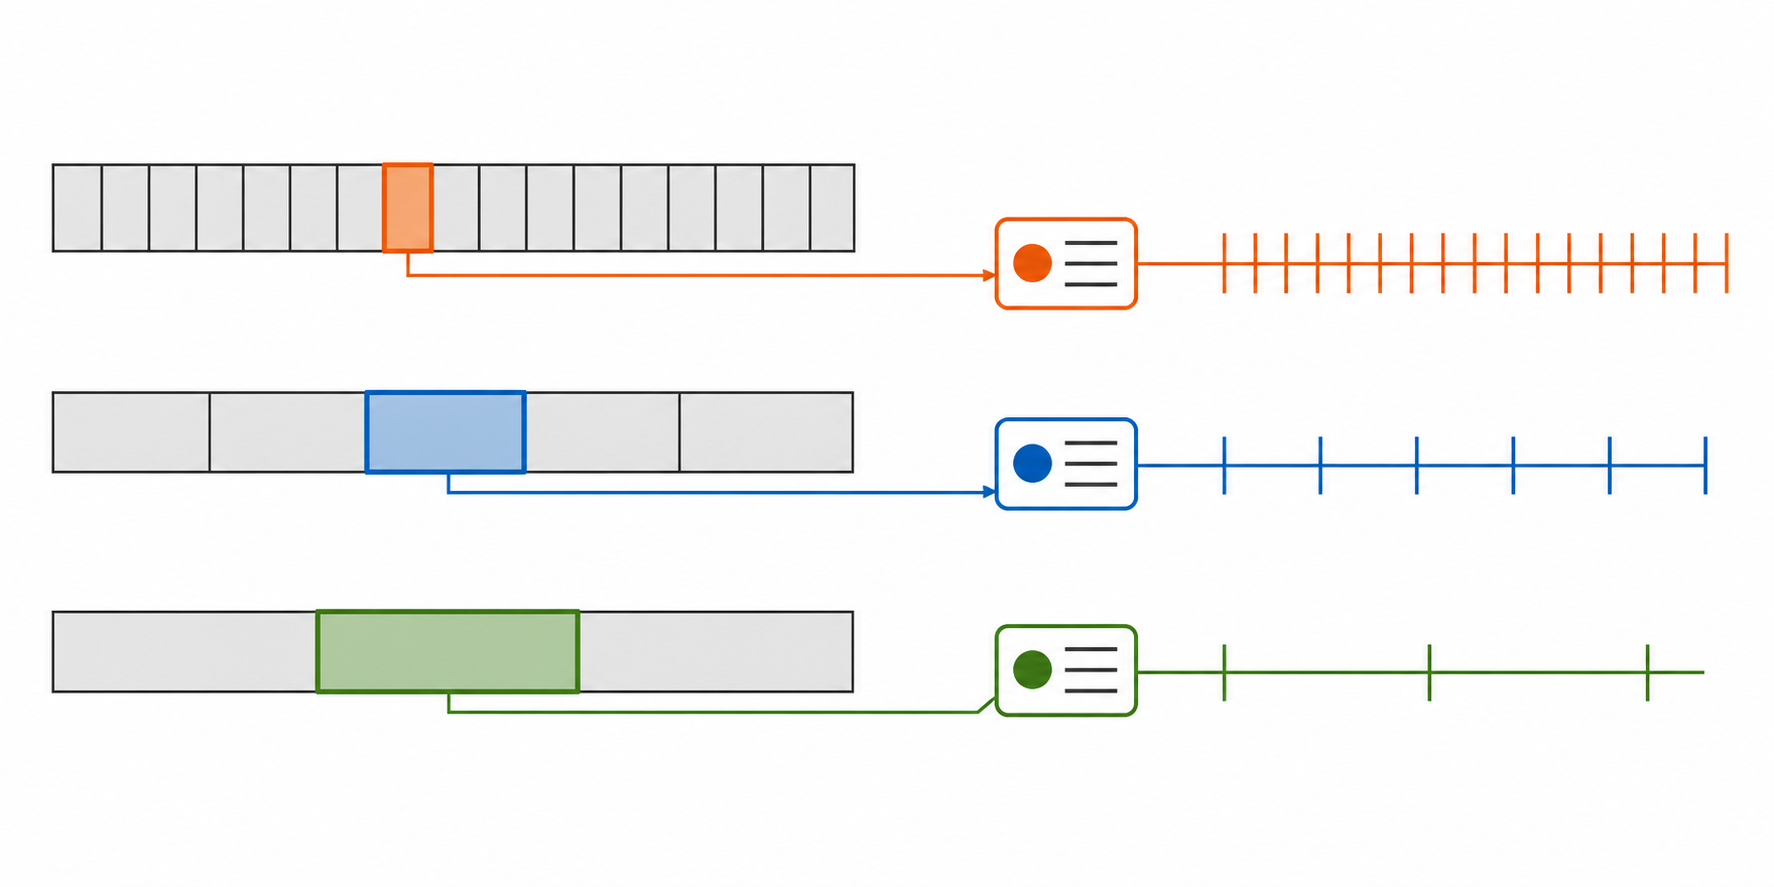
\includegraphics[width=0.93\linewidth,trim=0 65 0 65,clip]{figures/teaser_schedule_periodicity_v9_candidate.png}}
    \put(0,121){\footnotesize $L{=}16$}
    \put(0,73){\footnotesize $L{=}32$}
    \put(0,26){\footnotesize $L{=}64$}
  \end{picture}
  \caption{Qualitative measurement pipeline. From top to bottom, block length $L$
  grows while canvas extent stays fixed; color marks the one active block exposed
  to the recorder, and the right-hand ticks depict the boundary spacing visible
  through that window. Pulse and group counts are schematic, not quantitative
  evidence. Measured profiles and separations are in Figure~\ref{fig:period} and
  Table~\ref{tab:period}.}
  \label{fig:teaser}
\end{figure}

Across the matched arms, the detected period follows the configured block length;
separate non-power-of-two probes show the same recorder-observable pattern without
the nested-$32$ boundary relation. Neither result identifies a causal subtype.
The originally registered model-intrinsic branch was withdrawn after treatment
(amendment v3; Appendix~\ref{app:protocol}), and the measured candidate-$32$
signs are not values forced by nesting alone.

Our contribution is a two-layer reporting rule: specify before data which
outcomes the boundary-set composition makes reachable, then report separately
what the measured magnitudes show.  This separation prevents a recorder-defined
window from being interpreted as the mechanism that produced the tokens.  A
development control, matched block-length intervention, bootstrap stability
checks, negative probes, and content-sensitivity analysis support the
distinction on the tested beds; none establishes a mechanism across models or
schedules.

\section{Measurement and Design}\label{sec:method}

Core notation is defined here before it is used; Appendix~\ref{app:glossary}
retains the longer terminology crosswalk.

\begin{center}
\fbox{\begin{minipage}{0.94\linewidth}
\footnotesize
\textbf{Notation.} For decode $i$ and relative canvas position $r$,
$\ell_{i,r}$ is the recorded identity-lock time. Its positionwise median is
$m(r)$ and $d(r)=m(r{+}1)-m(r)$. For candidate period $P$,
$\mathcal B_P$ contains candidate boundary indices and $\mathcal I_P$ their
interior complement; $\operatorname{sep}(P)$ is the boundary-minimum minus the
interior-maximum of $d(r)$, and $P^*$ maximizes it. ``Canvas $96$'' denotes the
separate $96$-position probe bed. \textsc{BIN}$k$ denotes a restricted content
null with $k$ equally populated offset-rank strata.
\end{minipage}}
\end{center}

\paragraph{Model bed.}
We use an LLaDA-style masked dLLM at the LLaDA-8B-Instruct scale with a locally
registered checkpoint on GSM8K \citep{cobbe2021gsm8k}. Decoding uses temperature
$0$ and \texttt{remasking=low\_confidence}, the confidence-ordered parallel
decoding rule introduced for conditional masked language models and used by
LLaDA \citep{ghazvininejad2019maskpredict,nie2025large}. The main differential
fixes NFE at $48$ and uses the same $300$ questions. Its L32/NFE48 arm is a
frozen \emph{development control}: the registered contiguous
$\texttt{decode\_id}\in[345,645)$ subset of a pre-existing pool. The
L32/NFE32 content bed is separate and supports only Section~\ref{sec:content}.

\paragraph{Setup and protocol.}
Table~\ref{tab:setup} consolidates every bed and schedule. The headline length
metric is $d(r)=m(r{+}1)-m(r)$, the adjacent difference of median identity-lock
time. For content, the same lock-time ordering is compared with residualized
confidence under an explicit eight-stratum offset-rank null (BIN8; four-position
granularity), plus a same-amplitude \emph{position-fake}: confidence values are
assigned to positions to preserve amplitude while destroying the observed
content-to-position pairing. Intervals use cluster-bootstrap percentiles over
units \citep{davison1997bootstrap}; decode resampling preserves multiplicity.

\begin{table}[t]
\centering
\footnotesize
\setlength{\tabcolsep}{2.2pt}
\begin{tabular}{@{}>{\raggedright\arraybackslash}p{0.14\linewidth}
                  >{\raggedright\arraybackslash}p{0.25\linewidth}
                  >{\raggedright\arraybackslash}p{0.17\linewidth}
                  >{\raggedright\arraybackslash}p{0.20\linewidth}
                  >{\raggedright\arraybackslash}p{0.16\linewidth}@{}}
\toprule
Element & Measured arms & L32 control & Non-nested probes & Content bed \\
\midrule
Canvas / NFE & $256/48$ & $256/48$ & $96/48$ & $256/32$ \\
$L$; per-block steps & $16:[4]{\times}8+[2]{\times}8$; $64:[16,16,8,8]$ & $32:[8]{\times}4+[4]{\times}4$ & $24:[12]{\times}4$; $48:[24]{\times}2$ & $32$ \\
Questions & same $300$ & contiguous $[345,645)$, $n{=}300$ & same $300$ & GSM8K \\
Candidate grid & $\{8,16,32,64\}$ & $\{8,16,32,64\}$ & \shortstack[l]{$\{8,16,24,$\\$32,48,64\}$} & --- \\
Resampling & period $B{=}2000$; stability/sign $B{=}1000$ & period $B{=}2000$ & period $B{=}2000$ & interval $B{=}500$; null $R{=}2000$ \\
\bottomrule
\end{tabular}
\caption{Unified configuration. All beds use the same model family, task,
temperature, and remasking rule. The control's contiguous $[345,645)$ subset is
not part of the non-nested probes. Those two arms form a separate canvas-$96$
setup with $n{=}300$, NFE $48$, the displayed schedules and grid, and $2{,}000$
cluster-bootstrap replicates. NFE denotes total function evaluations. At fixed
total NFE, changing the partition also changes the required per-block step
allocation; the design is therefore a composite intervention and does not isolate
an allocation effect.}
\label{tab:setup}
\end{table}

\paragraph{Identity-lock time.}
For decode $i$, relative canvas position $r$, and recorded step $s$, let
$x_{i,r,s}$ be the predicted token and $x^f_{i,r}$ its final value. We define
\begin{equation}
\ell_{i,r}=\min\{s:x_{i,r,t}=x^f_{i,r}\ \text{for every recorded }t\ge s\}.
\label{eq:lock}
\end{equation}
Thus, $\ell_{i,r}$ is the earliest recorded step after which the token identity
never changes again. The position profile is $m(r)=\operatorname{median}_i
\ell_{i,r}$ and its adjacent difference is $d(r)=m(r+1)-m(r)$. All analysis uses
relative generated-canvas position, not prompt position.

\paragraph{Min--max period separation.}
For each candidate period in the registered grid (Table~\ref{tab:period}), define the candidate boundary set
$\mathcal B_P=\{r:r\bmod P=P-1\}$ and interior $\mathcal I_P$ as its complement.
The registered estimator is
\begin{equation}
\operatorname{sep}(P)=\min_{r\in\mathcal B_P}d(r)
-\max_{r\in\mathcal I_P}d(r),\qquad
P^*=\arg\max_P\operatorname{sep}(P).
\label{eq:sep}
\end{equation}
Exact ties select the first (smallest) period in the ordered registered grid.
Positive separation requires every candidate boundary jump to exceed every
interior jump. On a strictly $L$-supported profile it penalizes divisors with
false boundaries and multiples that leave true boundaries inside; without that
condition it is not a general divisor/multiple guarantee. A period is detected
only under the conjunction $\operatorname{sep}(P^*)>0$ and a cluster-bootstrap
modal period equal to $P^*$ with mode fraction at least $0.95$. The same
conjunction classifies each bootstrap readout below. We resample the $300$
decodes with replacement, preserving multiplicity, for $B{=}2{,}000$ replicates.

\paragraph{Selection stability and its honest reading of ``no misses.''}
Two resampling readouts are reported. First, a \emph{joint paired cluster
bootstrap} resamples a shared index set of the $300$ decodes once and applies the
same indices to all five arms (the matched three plus the two canvas-$96$
probes), so the headline is tested as a \emph{cross-arm relation} on shared
questions rather than as five independent marginals. Across $B{=}2{,}000$
replicates (seed $20260824$),
$\Pr[P^*_{16}{=}16\wedge P^*_{32}{=}32\wedge P^*_{64}{=}64]=1.0000$;
each of all five arms also has marginal $\Pr[P^*{=}L]=1.0$
(Table~\ref{tab:artifacts}).
Second, we report the probability that the detection rule actually fires,
$\Pr[\operatorname{sep}(L)>0]$, instead of the ``$0$ misses'' language.
Table~\ref{tab:fpr} consolidates this readout across all five arms. Because the
lock times are integer (temperature $0$), the min--max separation is an
integer-valued extremum of integer medians, so the bootstrap lower bound can sit
exactly at the point estimate and ``$0$ misses'' reflects discrete selection
stability rather than an absence of error. We therefore do not read a
$0/2{,}000$ miss count as ``no false detections.''

Because $\operatorname{sep}$ is an extremum statistic, we also report a
\emph{non-extremal} robustified comparison: a rank-sum (Mann--Whitney $U$)
separation between candidate-boundary and candidate-interior values of $d(r)$.
Its argmax period equals $L$ on \emph{all five} arms, including the L32 control
where the min--max separation was weakest; the per-arm statistics are in
Table~\ref{tab:fpr} and their provenance in Table~\ref{tab:artifacts}. A
quantile-based separation survives only on L64 and L48 and selects multiples
otherwise, which we report honestly as partial rather than as a full vote for
the extremum statistic.

\begin{table}[!b]
\centering
\footnotesize
\setlength{\tabcolsep}{2.7pt}
\begin{tabular}{@{}>{\raggedright\arraybackslash}p{0.31\linewidth}ccccc@{}}
\toprule
Readout & L16 & \shortstack{L32\\control} & L64 & \shortstack{L24\\probe} &
\shortstack{L48\\probe} \\
\midrule
$\Pr[\operatorname{sep}(L)>0]$, joint bootstrap & $1.0$ & $0.8805$ &
$0.9995$ & $0.999$ & $1.0$ \\
Rank-sum $z$ at $L$ & $13.9$ & $8.3$ & $4.4$ & $3.9$ & $2.0$ \\
Wrong-candidate fire rate, original three-bed probe & $0.0$ & $0.0$ & $0.0$ &
--- & --- \\
\bottomrule
\end{tabular}
\caption{Selection stability and non-extremal robustness (not a false-positive
rate). The first row uses one $B{=}2{,}000$ joint paired bootstrap and reports
how often the conjunction $\operatorname{sep}(L)>0$ and mode fraction
$\ge0.95$ fires. The L32 control's $0.8805$ is the weakest arm and appears
alongside the perfect modal-argmax relation. The second row is the
Mann--Whitney comparison, whose maximizing candidate is $L$ on every arm. The
final row is a separate $B{=}1{,}000$ in-place wrong-candidate diagnostic for
the original three beds: its zeros follow from negative point estimates and
are not fresh-null false-positive rates. Within an arm, cells share draws.
Provenance is in Table~\ref{tab:artifacts}.}
\label{tab:fpr}
\end{table}

\paragraph{Replication accounting.}
Table~\ref{tab:setup} is the complete resampling inventory. Period selection and
its interval share one draw, whereas the sign and stability checks use separate
draws; Table~\ref{tab:period} identifies the shared readouts. Uncounted values are
observed-data point estimates; artifacts are in Table~\ref{tab:artifacts}.

\paragraph{Matched intervention and scope.}
The two treatment arms and frozen development control are in
Table~\ref{tab:setup}. At fixed total NFE, changing the partition necessarily
changes per-block step allocation, so the treatment is
partition-plus-required-allocation. A within-arm rank transform preserves
$P^*{=}L$ and each candidate-$32$ sign on all five tested block-length arms,
including the non-power-of-two $L{=}24$ and $L{=}48$
(Table~\ref{tab:artifacts}); a uniform-allocation arm was not registered. The
result therefore identifies a recorder-output association with the composite
partition-plus-allocation schedule, not which component places or scales the
boundary. A factorial allocation/partition intervention is future work.

\paragraph{Registration and two-layer reachability.}
The estimator and detection rule were fixed before treatment, but amendment v3
withdrew the model-intrinsic decision branch after treatment; the timestamped
chronology is in Appendix~\ref{app:protocol}, Table~\ref{tab:timeline}. The
canvas-$96$ probes were registered separately before their execution. We therefore
report reachability at two layers. \emph{A priori}, nesting such as
$\mathcal B_{32}\subset\mathcal B_{16}$ determines set composition but not the
sign of $\operatorname{sep}(32)$. \emph{From events}, the observed magnitude
ordering gives $\operatorname{sep}(32)=-2$ on L16 and a negative value on L64.
Thus a recorder-observable fixed-$32$ component is not detected under these
active-block regimes; this does not identify model-intrinsic or sampler-state
causes. The exact loci and synthetic condition are consolidated in
Table~\ref{tab:negative}; the legacy verdict labels remain only in
Appendix~\ref{app:glossary}.

\paragraph{Separately conditioned content analysis.}
On the separate L32/NFE32 bed, BIN8 permutes confidence within eight
equally-populated offset-rank bins after a fixed nuisance fit. The initial
confidence $\texttt{conf0}$ is read at the first recorded step of a position's
block, following confidence-ordered parallel decoding
\citep{ghazvininejad2019maskpredict,nie2025large}. This supporting diagnostic is
not a cross-block-length validation.

\section{Results}\label{sec:results}

\subsection{The detected period follows block length}\label{sec:main}

The development control recovers its known period, and both treatment arms move
to their respective block lengths (Figure~\ref{fig:period};
Table~\ref{tab:period}). Only the selected period has positive min--max
separation, and the bootstrap selects it in every replicate.
The paired cross-arm relation holds in all $2{,}000$ shared-cluster resamples,
while a rank-sum point estimator independently selects $P^*{=}L$ in all five
arms. Across the five arms, $P^*$ leads the best wrong candidate by $+2.0$ to
$+8.0$ $d$-units; four reach $5\%$ significance against the within-block null
(exact $p_{\rm margin}\le2.1\times10^{-2}$), while L24 is marginal at
$p_{\rm margin}=7.1\times10^{-2}$ (Table~\ref{tab:sep-null}). The alignment is
therefore not reproduced by within-block jitter under that registered grid.

\paragraph{Candidate $32$ under the active-block recorder.}
Table~\ref{tab:period} reports $\operatorname{sep}(32)=-2$ on the measured $L=16$
arm. The exact values in Table~\ref{tab:negative} show why: candidate-$32$
boundary values remain positive, but the measured odd-$16$ interior is larger.
The joint sign $\operatorname{sep}(16)>0\wedge\operatorname{sep}(32)<0$ holds in
all $1{,}000$ dedicated bootstrap replicates. Candidate $32$ is therefore not
detected at the recorder-observable layer on this bed. Nesting alone does not
force that sign, and the result says nothing about an unobserved model-intrinsic
or sampler-state component.

\begin{figure}[t]
  \centering
  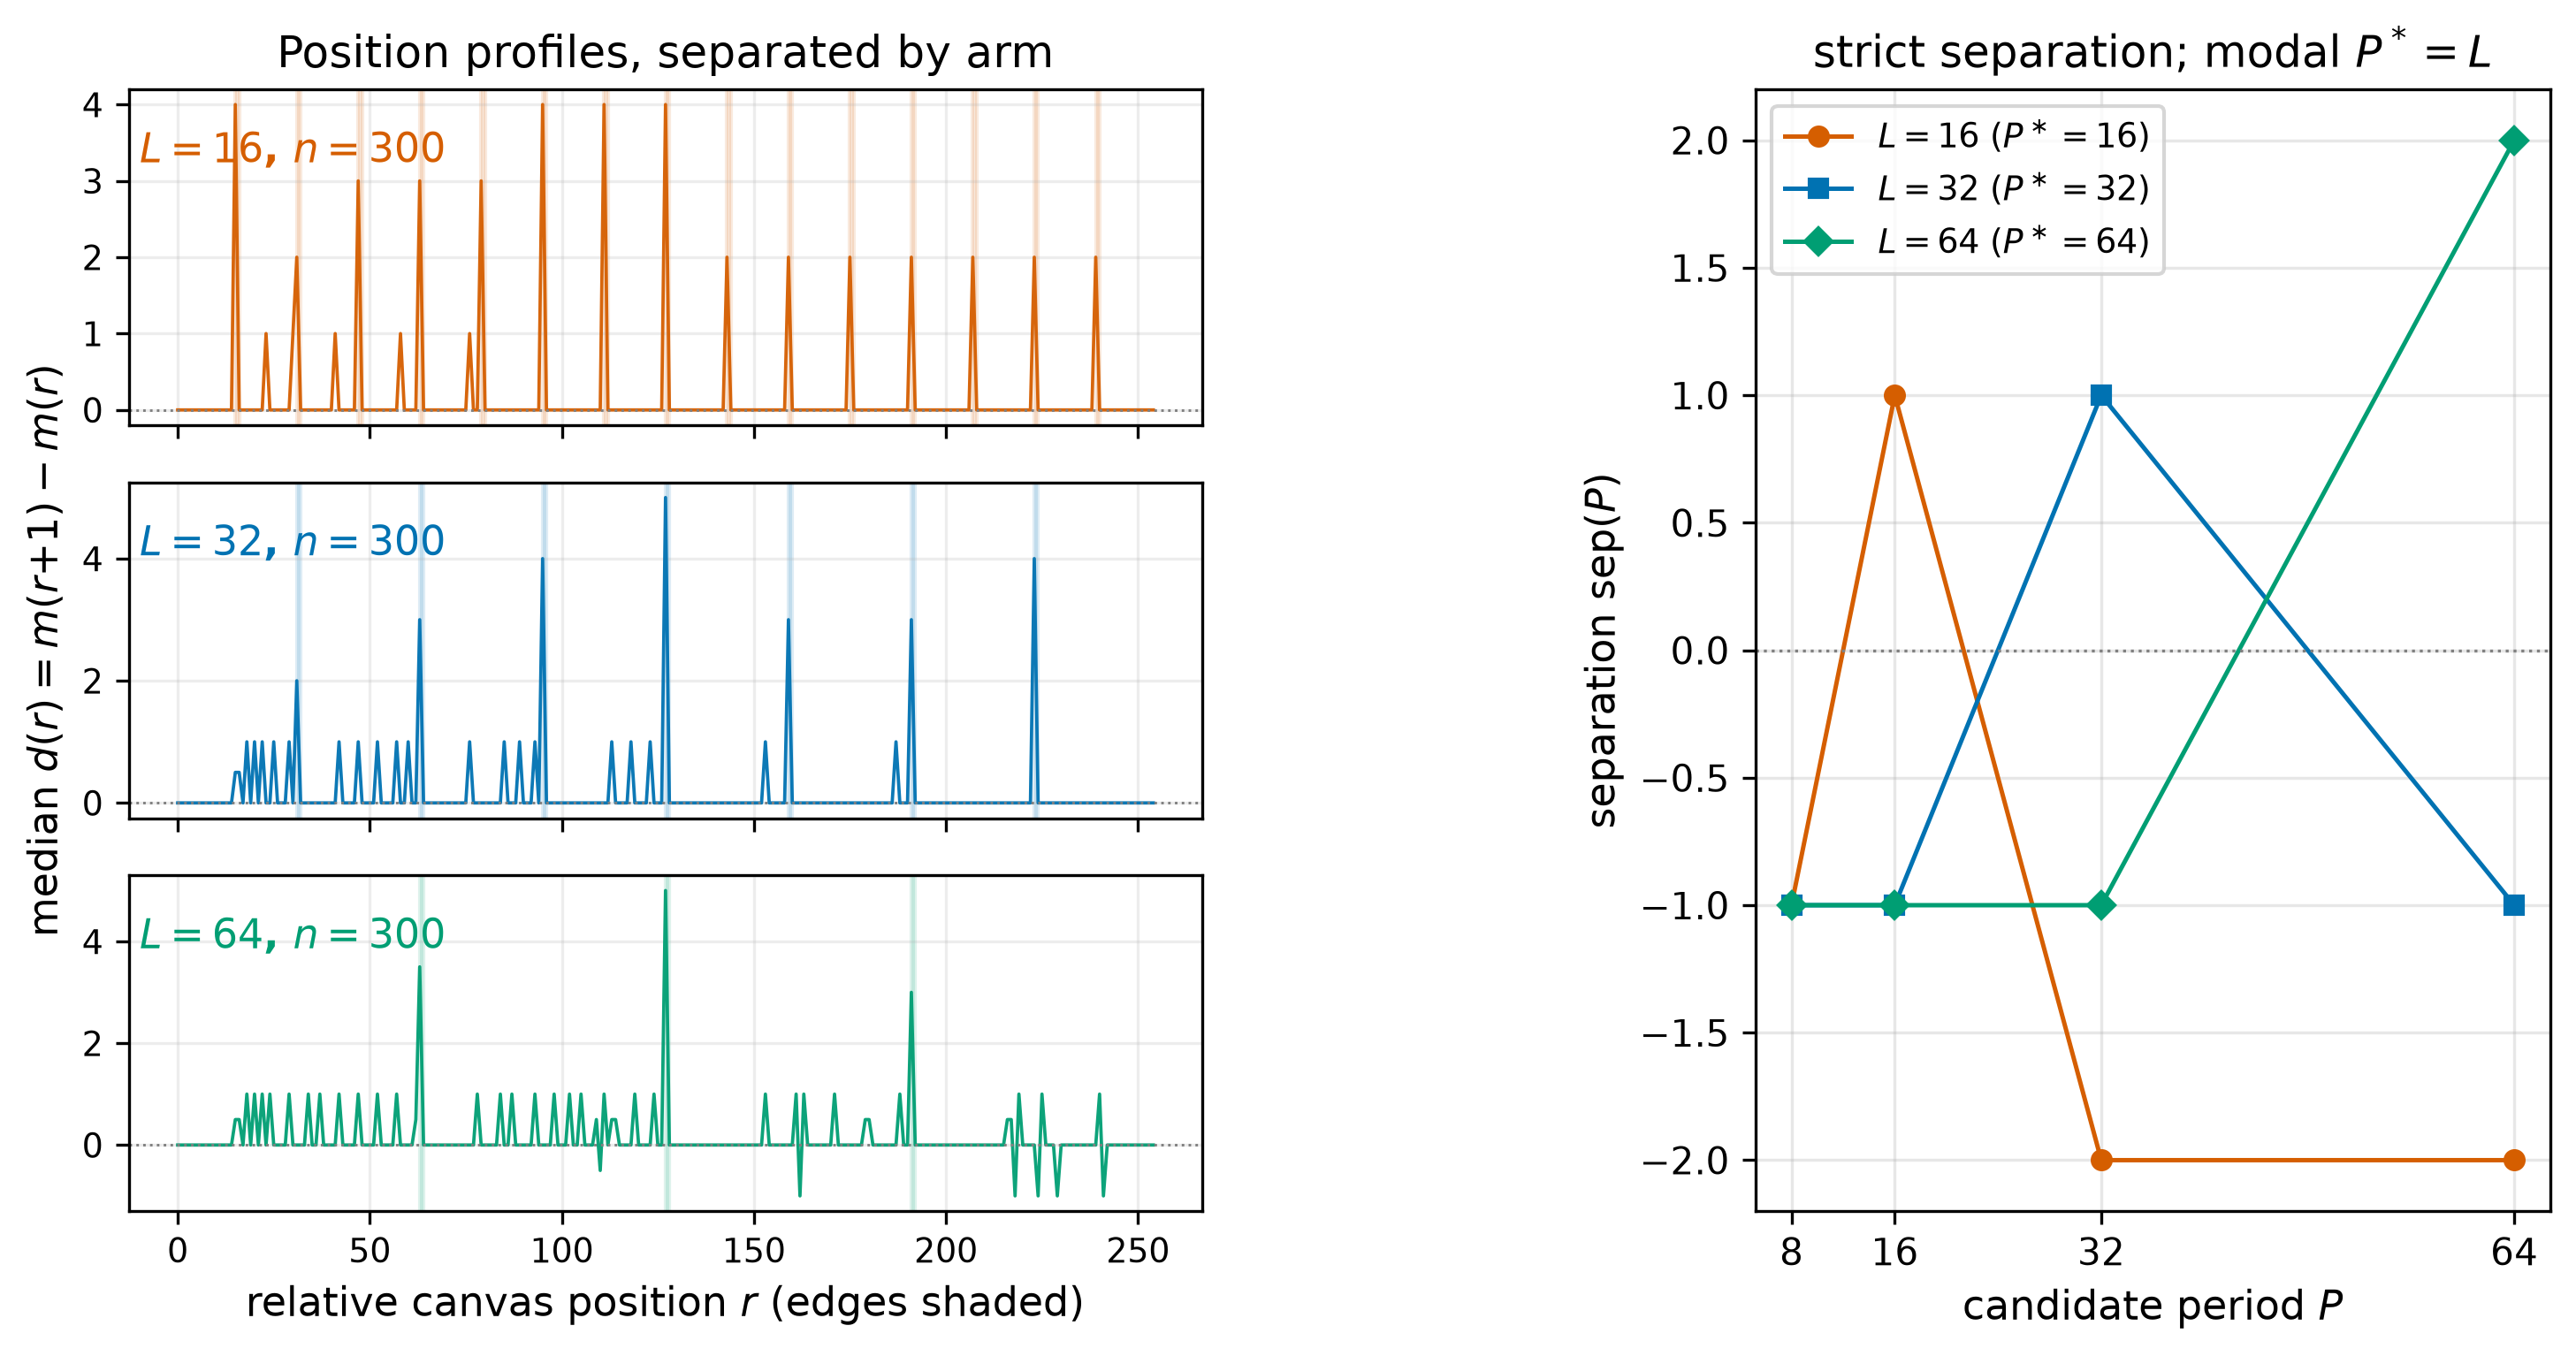
\includegraphics[width=\linewidth]{figures/period_follows_blocklen_dprofile.png}
  \caption{Data-derived differential result. Left: three stacked facets isolate
  the median adjacent-difference profile $d(r)=m(r{+}1)-m(r)$ for L16 (orange),
  the L32 frozen control (blue), and L64 (green), each from $n{=}300$ decodes;
  shaded ticks mark that arm's block edges. The control is the contiguous
  $\texttt{decode\_id}\in[345,645)$ subset. Right: only the matching candidate
  has positive separation in each arm. Regenerated by
  \texttt{scripts/r265\_fig\_dprofile\_overlay.py}; quantitative values come from
  the registered events, and the recorder-level comparison does not distinguish
  sampler from model mechanism.}
  \label{fig:period}
\end{figure}

\begin{table}[t]
\centering
\small
\setlength{\tabcolsep}{2.2pt}
\begin{tabular}{@{}lrrrrccccc@{}}
\toprule
& \multicolumn{4}{c}{$\operatorname{sep}(P)$} & & & & &  \\
\cmidrule(lr){2-5}
$L$ (source) & $P=8$ & $P=16$ & $P=32$ & $P=64$ &
\shortstack{$P^*$\\(mode frac.)} &
\shortstack{$\operatorname{sep}(P^*)$\\stability band$^{\dagger}$} &
\shortstack{$(\min_B,\max_I)$\\$@P^*$} &
\shortstack{$|B_{P^*}|$} &
\shortstack{$|I_{P^*}|$} \\
\midrule
$16$ (measured) & $-1$ & $+1$ & $-2$ & $-2$ & $16$ ($1.0$) & $[+1,+1]$ & $(+2.0,\,+1.0)$ & $15$ & $240$ \\
$32$ (control)  & $-1$ & $-1$ & $+1$ & $-1$ & $32$ ($1.0$) & $[\phantom{+}0,+2]$ & $(+2.0,\,+1.0)$ & $7$ & $248$ \\
$64$ (measured) & $-1$ & $-1$ & $-1$ & $+2$ & $64$ ($1.0$) & $[+1,+3]$ & $(+3.0,\,+1.0)$ & $3$ & $252$ \\
$24$ (probe) & --- & --- & --- & --- & $24$ ($1.0$) & $[+1.5,+4.0]$ & $(+5.0,\,+1.0)$ & $3$ & $92$ \\
$48$ (probe) & --- & --- & --- & --- & $48$ ($1.0$) & $[+4.0,+6.5]$ & $(+8.0,\,+1.5)$ & $1$ & $94$ \\
\bottomrule
\end{tabular}
\caption{Development-control, differential, and probe results. Each arm uses
$2{,}000$ cluster-bootstrap replicates; the mode fraction and percentile band
are paired readouts of the same draw. The $(\min_B,\max_I)$ columns report the
boundary minimum and interior maximum, followed by their observed set
cardinalities. Every arm selects its configured block length. Because lock times
are integer-valued, the bands diagnose selection stability rather than coverage:
L16 collapses to a point mass, while the L48 probe rests on one boundary location.
Tables~\ref{tab:setup}, \ref{tab:fpr}, \ref{tab:sep-null},
\ref{tab:spectral}, and~\ref{tab:content} give the complete resampling inventory
and separately budgeted checks; provenance is in Table~\ref{tab:artifacts}.}
\label{tab:period}
\end{table}

\begin{table}[H]
\centering
\footnotesize
\setlength{\tabcolsep}{4pt}
\begin{tabular}{@{}lcc@{}}
\toprule
Probe arm & Non-nested $\operatorname{sep}(32)$ & Disclosed marginal candidate \\
\midrule
$L{=}24$ probe & $-8.0$ & $P{=}48$: $-1.0$; band $[-3.0,0.0]$ \\
$L{=}48$ probe & $-7.5$ & --- \\
\bottomrule
\end{tabular}
\caption{Separate canvas-$96$ non-nested probes. Candidate $32$ is disjoint from
the $L{=}24$ boundaries. The L24 marginal cell concerns the mismatched $P{=}48$
candidate rather than detected $P^*{=}24$; the displayed percentile band is a
selection-stability diagnostic, not a coverage-valid interval.}
\label{tab:probes}
\end{table}

\FloatBarrier
\begin{table}[H]
\centering
\footnotesize
\setlength{\tabcolsep}{3.2pt}
\begin{tabular}{@{}lccrrr@{}}
\toprule
Arm & $P^*$ & $\operatorname{sep}(P^*)$ & $m_{\rm obs}$ & $p_{\rm sepL}$ & $p_{\rm margin}$ \\
\midrule
L16 (canvas 256) & $16$ & $+1.0$ & $+2.0$ & $5.0\times10^{-4}$ & $1.5\times10^{-3}$ \\
L64 (canvas 256) & $64$ & $+2.0$ & $+3.0$ & $5.0\times10^{-4}$ & $1.0\times10^{-3}$ \\
L24 (canvas 96) & $24$ & $+4.0$ & $+5.0$ & $5.0\times10^{-4}$ & $7.1\times10^{-2}$ \\
L48 (canvas 96) & $48$ & $+6.5$ & $+8.0$ & $2.3\times10^{-2}$ & $2.1\times10^{-2}$ \\
L32 control (canvas 256, NFE 48) & $32$ & $+1.0$ & $+2.0$ & $5.0\times10^{-4}$ & $1.0\times10^{-3}$ \\
\bottomrule
\end{tabular}
\caption{Separation-margin selectivity calibration. Each of $R{=}2{,}000$
replicates (seed $20260825$) permutes $d(r)$ within each true $L$-block,
including its edge index, then records the argmax candidate's top-minus-second
gap. Here $m_{\rm obs}=\operatorname{sep}(P^*)-
\max_{c\ne P^*}\operatorname{sep}(c)$ and the discrete exact
$p=(1+\#\{m_{\rm perm}\ge m_{\rm obs}\})/(R+1)$. The $p_{\rm sepL}$ column
tests $\operatorname{sep}(P^*)$ alone; $p_{\rm margin}$ is the
selection-controlled readout. Provenance and the original-gate size audit are
in Table~\ref{tab:artifacts} and Appendix~\ref{sec:selectivity-audit}.}
\label{tab:sep-null}
\end{table}

\FloatBarrier
\begin{table}[H]
\centering
\footnotesize
\setlength{\tabcolsep}{2.4pt}
\begin{tabular}{@{}>{\raggedright\arraybackslash}p{0.24\linewidth}
                  >{\raggedright\arraybackslash}p{0.25\linewidth}
                  >{\raggedright\arraybackslash}p{0.24\linewidth}
                  >{\raggedright\arraybackslash}p{0.20\linewidth}@{}}
\toprule
Measured class & Loci & $d(r)$ values & Readout \\
\midrule
L32 true-$32$ boundaries & \shortstack[l]{$[31,63,95,127,$\\$159,191,223]$} & $[2,3,4,5,3,3,4]$ & development control \\
L16 true-$16$ odd chain & \shortstack[l]{$[15,47,79,111,$\\$143,175,207,239]$} & $[4,3,3,4,2,2,2,2]$ & candidate-$32$ interior max $4$ \\
L16 would-be $\mathcal B_{32}$ & \shortstack[l]{$[31,63,95,127,$\\$159,191,223]$} & $[2,3,4,4,2,2,2]$ & boundary min $2$; $\operatorname{sep}(32)=-2$ \\
L64 mid-block $32$ & $[31,95,159,223]$ & L64: $[0,0,0,0]$; L32: $[2,4,3,4]$ & recorder-observable collapse \\
L64 true-$64$ & $[63,127,191]$ & L64: $[3.5,5,3]$; L32: $[3,5,3]$ & true boundary remains \\
\bottomrule
\end{tabular}
\vspace{2pt}

\begin{tabular}{@{}ccc@{}}
\toprule
Strict-support synthetic $L$ & Source periods & Selected $P^*$ \\
\midrule
$16$ & $\{8,16,32,48\}$ & $16$ for every source \\
$32$ & $\{8,16,32\}$ & $32$ for every source \\
$64$ & $\{8,16,32\}$ & $64$ for every source \\
\bottomrule
\end{tabular}
\caption{Consolidated negative evidence, reachability, and development check.
A priori, nested boundary sets determine membership but do not force the sign.
From events, L16 candidate $32$ has boundary minimum $2$ and interior maximum $4$;
the joint sign holds in $1{,}000/1{,}000$ bootstrap replicates. On L64, would-be
$32$ boundaries are recorder-observable interiors. The lower panel is a
development-only synthetic control: $P^*=L$ holds for the shown strictly
$L$-supported profiles, not for arbitrary residuals. The upper rows are
observed-data readouts from their arm samples, not additional replications.
Provenance is in Table~\ref{tab:artifacts}.}
\label{tab:negative}
\end{table}

\subsection{Separation and stability, not an effect-size power claim}

The central estimand is discrete period identity. On the observed samples,
positive min--max separation is a deterministic property of the recorded profiles;
the bootstrap then probes the stability of period selection to resampling decodes.
The selected period is stable under both the per-arm bootstrap and the joint
paired bootstrap that re-applies one shared question-index draw to all five arms
(Section~\ref{sec:method}); the detection rule fires in $0.88$--$1.0$ of
resamples across arms, with the L32 development control the weakest at
$\Pr[\operatorname{sep}(32){>}0]{=}0.8805$. A robustified non-extremal
rank-sum separation still selects $L$ on all five arms. This does not establish an
arbitrarily small effect or a universal period: it establishes stable selection
among the registered candidates on the stated bed, and the low-factor cells
($|B_{48}|{=}1$ on the L48 probe) temper any margin reading.
The L32 control also reuses a pre-existing contiguous $[345,645)$ pool and its
percentile stability band $[0,+2]$ touches zero (it is not a coverage-valid CI).
These three weaknesses are disclosed together; a fresh in-session L32 rerun is
GPU-gated future work.

\FloatBarrier
\subsection{A tested spectral residual family does not trigger on L16}\label{sec:nonnest}

For a nested candidate such as
$\mathcal B_{32}\subset\mathcal B_{16}$, a \emph{negative}
$\operatorname{sep}(32)$ is not evidence of absence: the extremum comparison
cannot recover every possible residual shape. An \emph{exploratory} (post-data,
not pre-registered) check therefore asks
whether a \emph{non-nesting} estimator recovers a residual source period that
$\operatorname{sep}$ misses. We use a DFT periodogram (non-nesting): for each
candidate $P$, $G(P)=\lVert\sum_r d(r)e^{-2\pi i r/P}\rVert/\lVert d\rVert$ is the
normalized spectral magnitude of the adjacent-difference profile at frequency
$1/P$, with a permutation null (shuffle $d(r)$ positions; $4{,}000$ replicates)
and family-wise $q_\mathrm{95}$ over all candidates. Harmonic testing follows
the periodogram tradition \citep{fisher1929harmonic}; our finite-grid threshold
is a bespoke single-step maximum over candidates, using the standard permutation
max-statistic construction \citep{nichols2002permutation}. We also run a direct
two-sample test of the two $L{=}16$-boundary subsets in
Table~\ref{tab:negative} (the odd-16 chain vs.\ the would-be-$\mathcal B_{32}$
positions), a reachable test of residual $32$-amplitude modulation.

\begin{table}[H]
\centering
\footnotesize
\setlength{\tabcolsep}{3.2pt}
\begin{tabular}{@{}lccccccc@{}}
\toprule
Case & $G(8)$ & $G(16)$ & $G(24)$ & $G(32)$ & $G(48)$ & $G(64)$ & $q_{95}@32$ \\
\midrule
\shortstack[l]{Synthetic, residual-$32$\\present} &
$3.58$ & $3.58$ & --- & $4.86$ & --- & --- & $1.74$ \\
Synthetic, no residual &
$4.01$ & $4.01$ & --- & $0.25$ & --- & --- & $1.75$ \\
\cmidrule(lr){2-8}
Real L16 measured &
$3.79$ & $3.70$ & $0.15$ & $0.23$ & $0.36$ & $0.18$ & $2.15$ (FW) \\
\bottomrule
\end{tabular}
\vspace{3pt}

\begin{tabular}{@{}>{\raggedright\arraybackslash}p{0.20\linewidth}
                    >{\raggedright\arraybackslash}p{0.34\linewidth}
                    >{\raggedright\arraybackslash}p{0.20\linewidth}
                    >{\raggedright\arraybackslash}p{0.18\linewidth}@{}}
\toprule
Supporting check & Statistic & Threshold / reference & Reading \\
\midrule
Injected residual & Residual-$32$ amplitude $0.5$ over comb-$16$ amplitude
$3.0$; $G(32){=}4.86$ & $q_{95}{=}1.74$ & fires \\
No-residual synthetic & $G(32){=}0.25$ & $q_{95}{=}1.75$ & null \\
Real L16 remaining grid & $G(24){=}0.15$, $G(48){=}0.36$,
$G(64){=}0.18$ & per-candidate $q_{95}\approx1.71$--$1.78$ & no residual candidate \\
Comb harmonic & $G(8)/G(16){=}1.000$ (pure comb), $1.024$ (real L16) &
$1.0$ reference ratio & recorder-comb harmonic \\
Power sweep & Amplitude $0.15$: no fire; $0.20$: fire; grid step $0.05$
($5.0\%$--$6.7\%$ of comb amplitude $3.0$) & $q_{95}$ above & transition bracketed \\
Odd-$16$ vs.\ would-be-$\mathcal B_{32}$ & Mean $|\Delta d|{=}0.036$;
permutation $p{=}1.0$ & $\alpha=0.05$ & no amplitude split \\
\bottomrule
\end{tabular}
\caption{Spectral (DFT) periodogram of the adjacent-difference profile
$d(r)$ --- an \emph{exploratory}, non-nesting check (Section~\ref{sec:nonnest}).
$G(P)$ is the normalized spectral magnitude at frequency $1/P$; ``fires''
means the $32$-component exceeds its permutation $q_{95}$ ($4{,}000$ replicates).
The upper panel completes the synthetic diagnostic grid and reports every real
candidate; the lower panel separates the supporting power, harmonic, and
two-sample checks from their interpretation. The synthetic residual fires,
whereas the comb-only synthetic and real L16 profile are null at the target
period. On real L16, no candidate in the tested grid is significant; only the
recorder-comb harmonics fire. The power sweep brackets sensitivity for the tested
sinusoidal family only, and the direct boundary-subset comparison finds no split.
Provenance is in Table~\ref{tab:artifacts}.}
\label{tab:spectral}
\end{table}

\textbf{Development control.} On the recorder-consistent synthetic grid, with a clean
sinusoidal residual-$32$ component overlaid on the $L{=}16$ comb,
$\operatorname{sep}$ returns $P^*{=}16$ (blind) while the spectral
$32$-component fires; on the no-residual synthetic comb, both are silent
(Table~\ref{tab:spectral}). This is a positive control for the tested sinusoidal
family, not validation against arbitrary residual shapes.

\textbf{Real L16 arm.} The tested candidate grid does not exceed its family-wise
threshold at $P=32$, and the boundary-subset test finds no amplitude split. The
registered power sweep brackets the tested-family transition and records its
amplitude range in Table~\ref{tab:spectral}. Hence the measured arm does not
trigger for this tested sinusoidal family and amplitude range; arbitrary residual
shapes are not ruled out (Table~\ref{tab:artifacts}).

\textbf{Canvas-$96$ non-nested probe (boundary disclosure).} On the separate
canvas-$96$ probe beds, candidate $32$ is \emph{non-nested} ($\mathcal
B_{32}\cap\mathcal B_{24}=\varnothing$), and the same estimator does not detect a
recorder-observable fixed-$32$ component without relying on the canvas-$256$
nesting relation. Table~\ref{tab:period} reports the two probe estimates,
their selected block lengths, and the disclosed marginal mismatched cell
(Table~\ref{tab:probes}); the probes used about $0.38$ GPU-h. This is a scoped
extension (canvas $96\ne256$), not a
replacement for the matched canvas-$256$ arms.

\FloatBarrier


The L64 mid-block reversal and its L32 comparator are reported without a separate
verdict vocabulary in the consolidated negative-evidence
Table~\ref{tab:negative}.

\subsection{A content association on a separate shared bed}\label{sec:content}

\paragraph{Estimand $\tau$.}
On the separate L32/NFE32 bed, one unit is a decode-block with resolved positions
$\mathcal R$; $c_r$ is initial confidence and $o_r=r\bmod32$ is block offset.
The estimand is the median per-unit rank association after residualizing confidence
on offset:
\begin{equation}
r_u=\frac{\sum_{p<q\in\mathcal R:\;\ell_p\ne\ell_q}
\operatorname{sgn}(\ell_q-\ell_p)\,\operatorname{sgn}(\tilde c_p-\tilde c_q)}
{\#\{p<q\in\mathcal R:\;\ell_p\ne\ell_q\}},
\qquad
\tilde c_r=\operatorname{rank}\!\big(\operatorname{rank}(c_r)-\hat\beta\,\operatorname{rank}(o_r)\big),
\label{eq:tau}
\end{equation}
Here the registered statistic fits $\hat\beta$ once on the observed data and
shuffles the resulting $\tilde c$ within offset-rank strata. A sensitivity check
instead refits $\hat\beta$ inside every permutation replicate. Earlier lock with
higher residualized confidence contributes $+1$.
Inference is rooted at decode clusters: the $500$-replicate interval resamples
decodes and carries their block units with multiplicity. The position-fake keeps
the observed amplitude but reassigns it to positions, destroying the observed
content--position pairing. This differently budgeted bed supplies supporting,
not cross-block-length, evidence.

\begin{table}[H]
\centering
\small
\setlength{\tabcolsep}{4pt}
\begin{tabular}{@{}>{\raggedright\arraybackslash}p{0.32\linewidth}
                    >{\raggedright\arraybackslash}p{0.23\linewidth}
                    >{\raggedright\arraybackslash}p{0.19\linewidth}
                    >{\raggedright\arraybackslash}p{0.18\linewidth}@{}}
\toprule
Quantity & Estimate / band & Null $q_{95}$ & Null readout \\
\midrule
Content-layer $\tau_{\rm res}$ & $0.2722$ $[0.2649,0.2812]$ & BIN16 $0.20235$ & $0/2000$ exceed \\
Refit-$\hat\beta$ sensitivity & $0.2722$ & BIN8 $0.13545$ & $0/2000$ exceed \\
Same-amplitude position fake & max. margin $+0.00979$ & observed margin $+0.12837$ & below observed \\
\bottomrule
\end{tabular}
\caption{Content-versus-structure result on the separate $L=32$, NFE-$32$
bed. The statistic $\tau$ is the median decode-block rank association between
earlier lock and higher confidence after offset residualization. BIN16 is the
load-bearing conservative, non-degenerate null; the per-replicate nuisance refit
is a separate BIN8 sensitivity and replays bit-exactly. Table~\ref{tab:content-audit}
reports the full granularity ladder and three-bucket one-flip classification.
This supporting analysis is not a cross-block-length experiment.}
\label{tab:content}
\end{table}


The full-granularity ladder in Table~\ref{tab:content-audit} is essential. The
observed association clears every non-degenerate restricted null through BIN16,
but matches the zero-power point mass at BIN32. Thus content association is
established at moderate granularity, never at the finest registered granularity;
the construction-specific BIN32 line is not interpreted as a lower bound. Its
behavior under $L\in\{16,64\}$ is unmeasured, and the two analyses are not
claimed to be mutually calibrated.


The full operational checklist and its strictly-$L$-supported scope are given in
Appendix~\ref{app:protocol}.

\section{Limitations}\label{sec:limits}

\begin{itemize}
  \item \textbf{Observation is not mechanism.} The active-block recorder cannot
  separate model-intrinsic state, sampler state, and recorder-observable state.
  Candidate $32$ is not detected only at the last layer under the tested regimes.
  \item \textbf{Registration history.} The estimator was selected with a failed
  development control before treatment, but the model-intrinsic decision branch
  was withdrawn after treatment. The non-nested probes have their own pre-run
  registration and a different $96$-position canvas.
  \item \textbf{Bed and grid.} Evidence covers one model family, one task, and the
  candidate grids in Table~\ref{tab:setup}; off-grid periods, other models, tasks,
  samplers, and untested block lengths are not covered.
  \item \textbf{Composite intervention.} Partition and required per-block step
  allocation vary together. Boundary location is measured; a distinct allocation
  effect on amplitude is not.
  \item \textbf{Boundary cardinality.} The min--max separation is an extremum
  statistic, so its support matters: on the probe arms the selected period rests
  on few measured boundary positions (the L48 probe has $|B_{48}|{=}1$), making
  its positive separation a single-locus readout rather than a stable margin. We
  report $|B_{P^*}|$ and $|I_{P^*}|$ per arm in Table~\ref{tab:period} for this
  reason.
  \item \textbf{Recorder and control arms.} A dual-recorder comparison that logs
  the same trajectory through active-block and full-canvas/passive instruments is
  GPU-gated future work; no cross-recorder result is claimed. A fresh in-session
  L32/NFE48 run is also GPU-gated: the present control reuses a pre-existing
  contiguous pool, has the lowest positivity ($0.8805$), and its percentile
  stability band touches zero.
  \item \textbf{Content scope.} The content association comes from one L32/NFE32
  bed and survives only through moderate null granularity (it is not established
  at the finest registered BIN32 granularity). Its behavior on the L16/L64 beds is
  not measured.
\end{itemize}

\section{Related Work}\label{sec:related}

Foundational discrete-diffusion work develops structured denoising,
reparameterization, density-ratio estimation, and simplified masked diffusion
\citep{austin2021structured,zheng2023reparameterized,lou2024discrete,shi2024simplified}.
These studies concern the model or sampler trajectory rather than an
active-block recorder perturbed at fixed model and NFE.

The nearest schedule-axis methods include fully parallel and
semi-autoregressive decoding \citep{gu2018nonautoregressive,wang2018semi},
confidence-ordered mask-predict and LLaDA-style decoding
\citep{ghazvininejad2019maskpredict,nie2025large,nie2026improved}, and variable
or reversible schedules \citep{li2025beyond,sun2026dystruct,wang2026reversible}.
Appendix Table~\ref{tab:closest} checks whether each work reports
position-resolved commit/lock timing and varies block length.  Wang et al.'s
positionwise cross-entropy periodicity is the closest partial precedent; the
setup differences do not support a field-wide absence claim.  Our content
analysis instead relates first-step confidence to later recorder lock ordering;
it is not a new remasking policy.

Measurement studies likewise show that probes inherit task-format confounds,
prompts can under-retrieve stored knowledge, and analysis choices shape the
reported representation \citep{sahoo2026linearprobes,jiang2020know,belinkov2018analysis}.
Construct validity therefore requires matching an instrument to its supported
target \citep{westreich2011table2fallacy}; preregistration separates planned
from outcome-contingent analysis but does not validate that target
\citep{nosek2018preregistration}.  Our two-layer record applies this principle
without the causal attribution of mediation analyses
\citep{stolfo2023mechanistic}.  Appendix Table~\ref{tab:nnpos} gives the
observation-window and scale comparison, including the distinct monitoring
example of \citet{feng2024monitoring}.  The post-treatment amendment remains
visible, the min--max result is restricted to strictly-$L$-supported candidates,
and the DFT control covers only the tested sinusoidal residual family.


\section{Conclusion}\label{sec:conclusion}

Under the tested active-block recorder, the detected identity-lock period follows
block length. Development controls, matched arms, non-nested probes, bootstrap
stability, and negative evidence support that recorder-level statement. They do
not distinguish model-intrinsic state, sampler state, and recorder observability.
The transferable result is the reporting rule: state what is reachable from set
composition before data, then separately state what the measured magnitudes show.
Calibrate position-decomposed measurements to the schedule that recorded them,
and do not infer a mechanism or cross-bed relation that the intervention did not
measure.

% P5_MAIN_TEXT_END
\label{p5:main-text-end}
\bibliography{refs}
\bibliographystyle{iclr2026_conference}

\appendix
\section{Protocol Chronology, Measurement Canon, and Sensitivities}\label{app:protocol}

\subsection{Registration chronology}

\begin{table}[H]
\centering
\footnotesize
\setlength{\tabcolsep}{3pt}
\begin{tabular}{@{}>{\raggedright\arraybackslash}p{0.16\linewidth}
                    >{\raggedright\arraybackslash}p{0.13\linewidth}
                    >{\raggedright\arraybackslash}p{0.62\linewidth}@{}}
\toprule
Timestamp & Status & Recorded event \\
\midrule
2026-08-20\newline 17:55 & Pre-data & Original registration filed before
any GPU submission. \\
2026-08-20\newline 18:09 & Pre-data & Amendment v2 replaced the failed
signed mean-difference score with the min--max estimator and registered the
detection rule. \\
2026-08-20\newline 23:07 & Treatment & Both treatment arms ran
($0.73$ GPU-h). \\
2026-08-21\newline 17:36 & Post-data & Amendment v3 withdrew the
model-intrinsic branch. \\
2026-08-21 & Pre-data (probe) & Non-nested canvas-$96$ probe registration
and amendments preceded its own run ($0.38$ GPU-h). \\
\bottomrule
\end{tabular}
\caption{Registration and amendment chronology. The estimator and detection rule
were fixed before treatment; the model-intrinsic decision branch was withdrawn
after treatment data were observed, so the chronology documents a scope change
rather than a pre-treatment mechanism verdict.}
\label{tab:timeline}
\end{table}

\newpage
\subsection{Artifact index}

\begingroup
\footnotesize
\setlength{\tabcolsep}{2pt}
\setlength{\LTpre}{3pt}
\setlength{\LTpost}{6pt}
\FloatBarrier
\begin{longtable}{@{}>{\raggedright\arraybackslash}p{0.17\linewidth}
                       >{\raggedright\arraybackslash}p{0.53\linewidth}
                       >{\raggedright\arraybackslash}p{0.24\linewidth}@{}}
\caption{Claim-to-artifact map. This is the sole table that prints
workspace-relative artifact paths; all narrative references point here. Full
provenance continues in \ap{evidence/claim_evidence_map.tsv},
\ap{evidence/method_provenance.tsv}, and
\ap{evidence/experiment_registry.json}.}\label{tab:artifacts}\\
\toprule
Claim / role & Workspace-relative artifact & SHA-16 \\
\midrule
\endfirsthead
\multicolumn{3}{@{}l}{\footnotesize\itshape Table~\thetable{} continued}\\
\toprule
Claim / role & Workspace-relative artifact & SHA-16 \\
\midrule
\endhead
\midrule
\multicolumn{3}{r@{}}{\footnotesize\itshape Continued on next page}\\
\endfoot
\bottomrule
\endlastfoot
L32 development control & \ap{results/blocklen_probe/G0_VERDICT_r3.json} & \ap{984b4ff92fe462ad} \\
L16/L64 period & \ap{results/r29_l16l64_sawtooth.json} & \ap{d462dff346604321} \\
Cross-arm bootstrap, rank-sum, stability bands & \ap{results/r295_joint_bootstrap_extremum_robust.json} & \ap{9a40c56c7c7a8243} \\
Within-block selectivity gate and size audit & \ap{results/decomposition_control_r314/r316_sep_withinblock_permnull.json}; \ap{results/decomposition_control_r314/r320_margin_selectivity.json} & \ap{f623432c139e440c}; \ap{e7d1c3115253589e} \\
Boundary/interior cardinalities & \ap{results/decomposition_control_r314/r316_bcardinality_per_arm.json} & \ap{e3a1c7b2b3c6915a} \\
Content statistic and interval & \ap{results/r10_poslevel_gates/r10_poslevel_gates_v2.json} & \ap{0af4f3c03e6c6f6d} \\
Content null ladder & \ap{results/r274_bin1632_null_ext.json} & \ap{b5d91fdc0b827018} \\
Per-permutation nuisance refit & \ap{results/r259_beta_recompute/r259_beta_recompute.json} & \ap{d3b27b3c87c924ce} \\
Bit-exact nuisance-refit replay & \ap{results/r259_replay_B/r259_replay_B.json} & \ap{85b875d858d0db19} \\
One-flip three-bucket classification & \ap{results/r311_oneflip/r311_oneflip.json} & \ap{47735637e3777a3d} \\
Position-fake control & \ap{results/r14_margin_sweep/r14_margin_sweep.json} & \ap{91da8f8b91a6b6b9} \\
L16 measured nested-candidate check & \ap{results/r58_z1b_L16_truepair.json} & \ap{10530a1b478ff492} \\
L64 mid-block comparison & \ap{results/r58_z2b_l64_neg_evidence.json} & \ap{470908f1400e7a1c} \\
Reachability table & \ap{results/r147_reachability_table/r147_reachability_table.json} & \ap{52a983b1c2fade9e} \\
Strict-support synthetic diagnostic & \ap{results/r147_entailment_demo/r147_entailment_demo.json} & \ap{ee4f1ad85d5492a2} \\
Spectral family and power grid & \ap{results/r259_non_nesting_spectral/r259_non_nesting_spectral.json}; \ap{results/r267_spectral_power_table.json} & \ap{a1b52a418ace4e07}; \ap{33768616bfa41ecc} \\
Rank-transform sensitivity & \ap{results/r265_rank_transform_invariance.json}; \ap{results/r299_orthogonal_separation_r299.json} & \ap{f1760ce13789a67d}; \ap{d90a4d56635f3771} \\
Figure~\ref{fig:period} manifest & \ap{results/r265_fig_dprofile_manifest.json} & \ap{40079e3c19996a01} \\
Control subset and row checks & \ap{results/r269_l32_control_subset_checks.json} & \ap{e5455d953fad8367} \\
Cross-environment reproduction & \ap{results/r269_estimator_byte_and_arm_recheck.json} & \ap{2c5f824c0ef215db} \\
Image-generation audit & \ap{build/image_generation_record.json} & \ap{c019dbf2309f460b} \\
\end{longtable}
\endgroup

\subsection{Measurement canon}\label{sec:canon}

For blockwise decoding observed through an active-block recorder, a
position-resolved analysis should:
\begin{enumerate}
  \item record block length, per-block steps, and generated-canvas coordinates;
  \item calibrate within-block windows to the generating run rather than a fixed
  model constant;
  \item report reachability twice: \emph{a priori}, what estimator algebra and
  boundary-set composition imply; \emph{from events}, what the measured magnitude
  ordering implies. In particular,
  $\mathcal B_{32}\subset\mathcal B_{16}$ does not force
  $\operatorname{sep}(32)\le0$;
  \item perturb the schedule when attributing a position-resolved diagnostic;
  \item test content claims against a structure-preserving null and report its
  granularity; and
  \item mark cross-bed relationships unmeasured until the corresponding
  intervention is run.
\end{enumerate}
This is a measurement canon, not a mechanism claim. The registered estimator
returns $P^*=L$ on the displayed \emph{strictly $L$-supported} profiles:
non-degenerate jumps occur on all $L$ boundaries and no $L$-multiple's
exclusive-boundary residual outscores the $L$-boundary minimum. It is not a
guarantee for arbitrary residual profiles, and identifying commit internals would
require instrumentation of sampler-state transfer.

\subsection{Selectivity disclosure (permutation-gate size audit)}
\label{sec:selectivity-audit}

\paragraph{Original-gate size.}
The original within-block threshold was anti-conservative. Across the five arms,
$10/25=40\%$ of wrong candidates (non-true-$L$ grid points) were flagged as
detected, so the nominal family-wise error of at most $5\%$ was not realized.
Table~\ref{tab:gate-audit} gives the per-arm audit. The cause is that
edge-including within-block permutation destroys the non-target global
level/trend structure of $d(r)$, shifting the null downward and loosening the
threshold.

\paragraph{Corrected margin and cross-condition red-team.}
Table~\ref{tab:sep-null} replaces that level gate with the top-minus-second
separation margin and a discrete exact $p$. As a known-clean red-team, globally
(cross-block) shuffling the same $d(r)$ constructs a structureless reference.
The corresponding probabilities are consolidated in
Table~\ref{tab:gate-audit}: four of five cross-condition checks are below $5\%$
and L24 is again marginal. This supports genuine schedule-aligned structure
rather than within-profile jitter. A genuinely clean arm has no blocks to
permute, however, so this red-team is a cross-condition comparison, not a
per-arm data-shuffle false-positive rate.

\begin{table}[H]
\centering
\footnotesize
\setlength{\tabcolsep}{6pt}
\begin{tabular}{@{}lcc@{}}
\toprule
Arm & Original-gate wrong candidates & Cross-condition $p_{\rm margin}$ \\
\midrule
L16 & $4/5$ & $5.0\times10^{-4}$ \\
L64 & $3/5$ & $2.0\times10^{-3}$ \\
L24 & $0/5$ & $5.5\times10^{-2}$ \\
L48 & $0/5$ & $1.8\times10^{-2}$ \\
L32 control & $3/5$ & $1.5\times10^{-3}$ \\
\midrule
Aggregate & $10/25$ ($40\%$) & $4/5$ below $5\%$ \\
\bottomrule
\end{tabular}
\caption{Selectivity-gate audit by arm. The original threshold flags
$10/25$ wrong candidates, whereas the cross-condition margin red-team is below
$5\%$ in four of five arms; L24 is marginal. These cross-condition probabilities
are not per-arm data-shuffle false-positive rates.}
\label{tab:gate-audit}
\end{table}

\paragraph{Reporting rule.}
Any threshold-type permutation gate used here for selectivity reports three
quantities together: the wrong-candidate hit rate, a known-clean-arm or explicit
cross-condition check, and the discrete exact $p$. The $10/25$ audit and the
margin correction therefore accompany every selectivity claim based on this
within-block gate.

\subsection{Three-part evidence decomposition}\label{sec:novelty}

For auditability, we separate the recorder-relative object $d(r)$, the
pre-treatment min--max decision procedure, and the scoped empirical finding that
$P^*$ follows $L$ on the tested recorder beds. The shared-cluster bootstrap and
rank-sum check support the decision procedure; the non-nested canvas-$96$ probes
bound the empirical finding. Table~\ref{tab:artifacts} maps each component to
its verifier. This decomposition is a falsification aid, not three independent
novelty claims or a mechanism attribution.

\subsection{Content accounting and null granularity}

\begin{table}[H]
\centering
\small
\setlength{\tabcolsep}{4pt}
\begin{tabular}{@{}>{\raggedright\arraybackslash}p{0.34\linewidth}
                    >{\raggedright\arraybackslash}p{0.25\linewidth}
                    >{\raggedright\arraybackslash}p{0.33\linewidth}@{}}
\toprule
Accounting / sensitivity check & Recorded value & Interpretation \\
\midrule
Content-resolved block-units & $6{,}178$ of $6{,}274$ candidates &
Terminal-resolved units excluded \\
Resolved comparable pairs & $1{,}571{,}854$ & Both positions resolve \\
Within-unit support & Median $4$ distinct locks; median resolved-pair fraction
$0.575$ & Unit-level order is observed \\
Resampling & $\texttt{n\_boot}{=}500$; $\texttt{R\_null}{=}2000$ &
Decode-cluster interval and restricted null \\
K-ladder restricted-null $q_{95}$ & $K{=}1$: $0.00486$; BIN4 $0.09276$;
BIN8 $0.14384$; BIN16 $0.20235$; BIN32 $0.27221$ (point mass) & With
$\tau_{\rm res}{=}0.2722$, margins at $K{=}1$, BIN4, BIN8, and BIN16 are
$0.26735$; $0.17945$; $0.12837$; $0.06986$; BIN32 is zero-power by construction and
carries no lower-bound reading \\
Nuisance-$\hat\beta$ sensitivity & Refit inside each BIN8 replicate:
$q_{95}{=}0.13545$; fixed-fit BIN8 $q_{95}{=}0.14384$ & $0/2000$ exceedances;
bit-exact replay. BIN16 remains the load-bearing conservative non-degenerate arm \\
One-flip sensitivity ($1/n_{\rm selected}$) & $n_{\rm selected}{=}6178$;
all $6178$ residual-sign flips give $\Delta{=}0$ & \textsc{degenerate},
by construction; no pass claim. The null-specification ladder, not this identity
arm, carries the sensitivity conclusion \\
\bottomrule
\end{tabular}
\caption{Unit accounting and restricted-null sensitivity for
Table~\ref{tab:content}. A block-unit is rooted in its decode cluster; decodes are
resampled with multiplicity. The registered line fits the nuisance slope once;
the displayed sensitivity refits it inside each replicate. One-flip granularity
is $1/n_{\rm selected}$, not permutation spacing $1/R$. Under the three-bucket
contract, maximum single-point effect $\phi=0$ is \textsc{degenerate}
(by construction) and carries no pass/fail claim; $0<\phi\le$ margin would pass
and $\phi>$ margin would fail. BIN32 is likewise zero-power by construction.
The full sweep therefore limits the positive finding to moderate granularity.
Provenance is in Table~\ref{tab:artifacts}.}
\label{tab:content-audit}
\end{table}

\subsection{Closest-work setup comparison}

\begingroup
\small
\setlength{\tabcolsep}{2.2pt}
\setlength{\LTpre}{3pt}
\setlength{\LTpost}{6pt}
\setlength{\LTcapwidth}{\linewidth}
\FloatBarrier
\begin{longtable}{@{}>{\raggedright\arraybackslash}p{0.14\linewidth}
                    >{\raggedright\arraybackslash}p{0.26\linewidth}
                    >{\raggedright\arraybackslash}p{0.17\linewidth}
                    >{\raggedright\arraybackslash}p{0.35\linewidth}@{}}
\caption{Row-wise setup comparison for the cited nearest work. Entries state the
object and observation window, the schedule/measurement action, and the resulting
contrast with this recorder audit, including whether each reports \emph{both} layers
of our two-layer rule (a-priori reachability \emph{and} from-events magnitude).
These scoped contrasts do not assert that an entire research area lacks schedule
diagnostics or mechanism analysis.}\label{tab:closest}\\
\toprule
Work & Object and observation window & Schedule action / measurement & Measurement-layer contrast used here \\
\midrule
\endfirsthead
\multicolumn{4}{@{}l}{\footnotesize\itshape Table~\thetable{} continued}\\
\toprule
Work & Object and observation window & Schedule action / measurement & Measurement-layer contrast used here \\
\midrule
\endhead
\midrule
\multicolumn{4}{r@{}}{\footnotesize\itshape Continued on next page}\\
\endfoot
\bottomrule
\endlastfoot
\citet{austin2021structured} & Structured discrete-state denoising; model/sampler trajectory & Schedule belongs to the formulation & Background; reports neither a-priori reachability nor from-events magnitude \\
\citet{zheng2023reparameterized} & Reparameterized text diffusion; generated trajectory & Reparameterizes a fixed generative process & Changes model parameterization; we hold the model fixed and perturb the recorder-facing partition \\
\citet{lou2024discrete} & Distribution-ratio estimation for discrete diffusion; likelihood/generation & Schedule supports the generative objective & Targets modeling/likelihood, not boundary-set reachability \\
\citet{shi2024simplified} & Simplified masked diffusion; model/sampler output & Simplifies the diffusion formulation & Supplies the masked-diffusion setup, not the two-layer recorder audit \\
\citet{li2025beyond} & Variable-length inference; whole-decode outcomes across lengths & Changes denoising length & Schedule change used for decoding; ours fixes total NFE over a block-partition co-movement \\
\citet{sun2026dystruct} & Bayesian dynamically structured decoding; evolving decode & Adapts decoding structure & Schedule is the method's action; ours treats it as a diagnostic perturbation \\
\citet{wang2026reversible} & Reversible diffusion decoding; revisable trajectory & Permits decisions to be revisited & Reversibility changes the trajectory; ours audits masked active-block events \\
\citet{sahoo2026linearprobes} & Hidden-state linear probe; language-model input/activations & Deconfounds measurement from format & Warns instrumentation confounds can induce a readout; reports measured magnitudes, not a-priori set composition \\
\citet{jiang2020know} & Prompt query of LM knowledge; output distribution & Optimizes prompts & Frames any measurement as a lower bound; distinguishes reachability from measured magnitude for facts \\
\citet{belinkov2018analysis} & Analysis/probing methods for representations; activations & Chooses analysis method & Choice of method changes what is measured; no recorder-window partition perturbation \\
\citet{feng2024monitoring} & Propositional probes of latent world states; activations & Monitors via probes & Shows recorded layer can diverge from behavior; does not perturb the recording window \\
\citet{stolfo2023mechanistic} & Causal-mediation attribution; internal states & Intervenes on internal states & Attributes mechanism; we do \emph{not} and report only recorder-level reachability \\
This work & Identity-lock adjacent difference; active-block event window & Matched block-length intervention plus required allocation & Separates a-priori set composition from from-events magnitude; does not claim mechanism \\
\end{longtable}
\endgroup

\begingroup
\footnotesize
\setlength{\tabcolsep}{3.2pt}
\setlength{\LTpre}{3pt}
\setlength{\LTpost}{6pt}
\setlength{\LTcapwidth}{\linewidth}
\begin{longtable}{@{}>{\raggedright\arraybackslash}p{0.17\linewidth}
                >{\raggedright\arraybackslash}p{0.30\linewidth}
                >{\raggedright\arraybackslash}p{0.12\linewidth}
                >{\raggedright\arraybackslash}p{0.35\linewidth}@{}}
\caption{Nearest-neighbor positioning against the closest conceptual
measurement works. Each prior operates on a different measured dimension; the
table states that relation and the checks already run on the recorder-window
period-separation dimension. Artifact paths and SHA-16 prefixes are in
Table~\ref{tab:artifacts}; this is not a mechanism attribution.}
\label{tab:nnpos}\\
\toprule
Closest conceptual work & Their measured dimension (claim) & Same dim.\ here? & Testable gap this recorder audit runs (already run) \\
\midrule
\endfirsthead
\multicolumn{4}{@{}l}{\footnotesize\itshape Table~\thetable{} continued}\\
\toprule
Closest conceptual work & Their measured dimension (claim) & Same dim.\ here? & Testable gap this recorder audit runs (already run) \\
\midrule
\endhead
\midrule
\multicolumn{4}{r@{}}{\footnotesize\itshape Continued on next page}\\
\endfoot
\bottomrule
\endlastfoot
\citet{jiang2020know} & Prompt-level QA recall/accuracy on factual knowledge; measurement as a lower bound on stored facts & No --- conceptual source of our two-layer split; their scale is knowledge retrieval & Differential separator, non-nested canvas-$96$ probes, and five-arm rank-transform invariance (Table~\ref{tab:artifacts}) \\
\citet{sahoo2026linearprobes} & Hidden-state probe AUROC/accuracy; confound driven by task format, collapsing after deconfounding & No --- deconfounds task format, not the recorder partition & Matched composite partition intervention plus a non-nested canvas-$96$ instrumentation self-check (Table~\ref{tab:artifacts}) \\
\citet{feng2024monitoring} & Propositional-probe AUROC for latent world states; recorded layer vs behavior divergence & No --- compares layer to behavior, does not perturb the recording window & Fixed model/NFE recorder-window perturbation, paired bootstrap, and rank-sum separation (Table~\ref{tab:artifacts}) \\
\end{longtable}
\endgroup

\section{Reproducibility and Artifact Map}\label{app:artifacts}

Execution cost, shard completion, and event-row validation are reported in
Table~\ref{tab:exec}, separately from provenance, so that spend is never conflated
with a completeness check. Every quantitative statement in the main text traces to
the on-disk artifacts in Table~\ref{tab:artifacts}; hashes are whole-file SHA-256
prefixes computed from the current workspace.

\textbf{Determinism.} Decoding uses temperature $0$ with
\emph{remasking=low\_confidence}; under the fixed decoding rule and fixed NFE
schedule, token selection is deterministic on a fixed canvas, so the identity-lock
profile $m(r)$ and its adjacent difference $d(r)$ are deterministic functions of
(model, checkpoint, seed, question set, NFE schedule). Min--max separation
$\operatorname{sep}(P)$, period selection, and every reported spectral value are
deterministic properties of these recorded profiles (only the bootstrap /
permutation-replicate quantities carry sampling randomness). Determinism is scoped
per (checkpoint, seed, question assignment, NFE schedule); cross-seed variance is
not the pre-registered estimand.

\textbf{Environment.} The registered analyses ran under Python 3.11.13, NumPy
2.4.6, pandas 2.3.1, PyArrow 21.0.0, PyTorch 2.7.1; the model is a locally
registered LLaDA-8B-Instruct-scale masked dLLM, blockwise decoded over GSM8K
(\citealt{cobbe2021gsm8k}), a fixed $300$-question canvas at $256$ positions and
$48$ total NFE per arm. The checkpoint is a private local artifact (registry per
the project evaluation ledger) and is \emph{not} byte-identical to the public
LLaDA-8B-Instruct release; we verify its magnitude is at the same scale but do not
assert release equivalence. The full manifest and core-script index are in
Table~\ref{tab:artifacts}.

\textbf{Cross-environment reproduction.} The estimator source was touched after
the submission manifest recorded its hash, so rather than assert equivalence we
re-derived every arm from raw events with the \emph{current} bytes in a second software
environment (Python 3.12.3, NumPy 2.5.2, pandas 3.0.5). All three arms reproduce
their sealed $\operatorname{sep}$ vectors and selected periods \emph{exactly}, so
the second-environment Table~\ref{tab:period} values equal the first-environment
values bit-for-bit and are not restated as a duplicate column. The complete
arm-by-candidate values and both estimator hashes are indexed in
Table~\ref{tab:artifacts}.

\textbf{Repro kit.} Seeds, question identities, the event schema, and a
one-command rebuild are provided for the off-GPU parts. Decode uses
$\texttt{seed}{=}20260820$ and the frozen question subset
$\texttt{decode\_id}\in[345,645)$. Every numeric readout can be regenerated from
the recorded-event schema with the indexed estimator and one-shot re-derivation
(Table~\ref{tab:artifacts}). The model checkpoint cannot be re-released without
authorization; an anonymous supplement of releasable events, scripts, and hashes
remains subject to provenance approval.

\begin{table}[H]
\centering
\footnotesize
\setlength{\tabcolsep}{2pt}
\begin{tabular}{@{}>{\raggedright\arraybackslash}p{0.19\linewidth}
                    >{\raggedright\arraybackslash}p{0.77\linewidth}@{}}
\toprule
Execution accounting & Recorded value \\
\midrule
Hardware & eight GPUs \\
Timing & $330$ running s $=0.73$ GPU-h; $130$ queueing s reported separately
and excluded \\
Shard completion & $L=16$: $4/4$; $L=64$: $4/4$ \\
Event-row check & $L=16$: $153{,}600=300\times512$;
$L=64$: $499{,}200=300\times1664$; $L=32$ control:
$268{,}800=300\times896$ rows for $\texttt{decode\_id}\in[345,645)$ of the
frozen NFE-$48$ pool \\
\bottomrule
\end{tabular}
\caption{Execution cost and completion checks for the two new treatment arms and
the frozen control subset. Cost is reported for the GPU submission that produced
the $L{=}16$ and $L{=}64$ arms; shard and event-row checks establish completion,
whereas the control arm reuses a pre-existing pool.}
\label{tab:exec}
\end{table}

\paragraph{AI-assisted preparation disclosure.}
Image generation produced qualitative Figure~\ref{fig:teaser}; the selected
candidate passed an element-level semantic audit and carries no measurements.
Figure~\ref{fig:period} remains data-derived. An AI assistant edited prose and
LaTeX; all claims, numbers, citations, and hashes were checked against the listed
evidence.

\section{Notation and Terminology}\label{app:glossary}

Table~\ref{tab:glossary} collects the estimator notation and verdict vocabulary;
Table~\ref{tab:beds} collects the bed names, the treatment variable, and the
content-layer terms. Each entry names the section that defines it.

\begingroup
\footnotesize
\setlength{\tabcolsep}{3pt}
\setlength{\LTpre}{3pt}
\setlength{\LTpost}{6pt}
\FloatBarrier
\begin{longtable}{@{}>{\raggedright\arraybackslash}p{0.22\linewidth}
                       >{\raggedright\arraybackslash}p{0.72\linewidth}@{}}
\caption{Estimator notation and legacy decision-table vocabulary; terms point to
their operative definition and do not attribute mechanism.}\label{tab:glossary}\\
\toprule
Term & Meaning (defining location) \\
\midrule
\endfirsthead
\multicolumn{2}{@{}l}{\footnotesize\itshape Table~\thetable{} continued}\\
\toprule
Term & Meaning (defining location) \\
\midrule
\endhead
\midrule
\multicolumn{2}{r@{}}{\footnotesize\itshape Continued on next page}\\
\endfoot
\bottomrule
\endlastfoot
$\ell_{i,r}$ & Identity-lock time: earliest recorded step after which decode
$i$'s token at relative position $r$ never changes again (Eq.~\eqref{eq:lock}). \\
$m(r)$, $d(r)$ & Per-position median lock time over decodes, and its adjacent
difference $m(r{+}1)-m(r)$ (Section~\ref{sec:method}). \\
$\mathcal B_P$, $\mathcal I_P$ & Candidate-$P$ boundary set
$\{r:r\bmod P=P-1\}$ and its complement, the candidate interior
(Section~\ref{sec:method}). \\
$\operatorname{sep}(P)$, $P^*$ & Min--max period separation
$\min_{\mathcal B_P}d-\max_{\mathcal I_P}d$, and its maximizing candidate
(Eq.~\eqref{eq:sep}). \\
\textsc{detected} & $\operatorname{sep}(P^*)>0$, bootstrap modal period $=P^*$,
mode fraction $\ge0.95$ (registered rule, Section~\ref{sec:method}). \\
\textsc{refuted} / \textsc{not-supported} & Measured $\operatorname{sep}(P)<0$
for a candidate that the decision table treated as refutable / for the
originally registered intrinsic-$32$ conjunct, whose branch was withdrawn
post-data (Table~\ref{tab:negative}). \\
\textsc{a-priori} layer & What follows from the estimator's algebra alone,
before data --- e.g.\ boundary-set nesting (Section~\ref{sec:method}). \\
\textsc{from-events} layer & What follows only once measured magnitudes exist ---
e.g.\ the sign of $\operatorname{sep}(32)$ (Section~\ref{sec:method}). \\
Strictly $L$-supported & Recorded profile with non-degenerate jumps on all
$L$-block boundaries such that no $L$-multiple's exclusive-boundary residual
outscores $L$'s boundary minimum (Section~\ref{sec:main}). \\
$G(P)$, perm.\ $q_{95}$, fam.\ $q_{95}$ & Normalized DFT magnitude of $d(r)$ at
frequency $1/P$; its per-candidate permutation $95$th percentile; the
family-wise version over all candidates (Section~\ref{sec:nonnest}). \\
\end{longtable}
\endgroup

\begin{table}[H]
\centering
\footnotesize
\setlength{\tabcolsep}{3pt}
\begin{tabular}{@{}>{\raggedright\arraybackslash}p{0.22\linewidth}
                    >{\raggedright\arraybackslash}p{0.72\linewidth}@{}}
\toprule
Term & Meaning (defining location) \\
\midrule
L16 arm, L64 arm & The two new matched treatment arms at block length
$16$ and $64$, NFE $48$ (Table~\ref{tab:setup}). \\
L32/NFE48 control & Frozen matched positive control at block length $32$,
NFE $48$: the registered $\texttt{decode\_id}\in[345,645)$ subset, $n{=}300$
(Sections~\ref{sec:method} and~\ref{sec:main}). \\
L32/NFE32 content bed & Separate, differently budgeted bed used only for the
content-association diagnostic (Section~\ref{sec:content}). \\
Partition-plus-required allocation & The composite treatment: changing the block
partition necessarily changes the per-block step allocation at fixed total NFE
(Table~\ref{tab:setup}). \\
Measurement-class label & \textsc{Period-Follows-Block-Length}: a post-data label stating that the detected
boundary period follows block length on the tested bed under the active-block
recording window; not a mechanism attribution
(Sections~\ref{sec:intro} and~\ref{sec:main}). \\
\textsc{BIN8} & Restricted null that permutes residualized confidence within $8$
equally populated offset-rank bins, preserving offset structure to
$4$-position granularity (Sections~\ref{sec:method} and~\ref{sec:content}). \\
$\texttt{conf0}$ & Position-$r$ initial confidence at block-commit: the model's
confidence for $r$ at the first recorded step of its block
(Section~\ref{sec:method}). \\
Block-unit; resolved position & One decode-block of the content bed; a position
whose lock time is defined and that never flips after lock. Terminal-resolved
units, which present no within-block pairwise order, are excluded
(Table~\ref{tab:content}). \\
$\tau$, $\tau_{\rm res}$ & Median over units of the per-unit rank association
between lock time and confidence; the offset-residualized (content-layer)
version (Eq.~\eqref{eq:tau}). \\
\bottomrule
\end{tabular}
\caption{Bed, treatment, and content-layer terms; the matched setting and separate
content bed remain distinct.}
\label{tab:beds}
\end{table}

\FloatBarrier
\end{document}
